\chapter{Metodologia do Trabalho}
    \section{Introdução}
        A nossa metodologia de trabalho foi uma adaptação da proposta de (Bittner, 2002)\cite{usecases}, ODP() e Scrum\cite{essentialscrum}. Tendo entendido o problema e o \textit{stakeholders} (primeira parte), Unimos a completeza e formalidade da definição de requisitos funcionais identificáveis por casos de uso e ODP para a concepção inicial do produto (segunda parte), inserindo esses conhecimentos num \textit{framework} de \textit{Scrum}, adaptado para o nosso contexto (terceira parte).
        
        \begin{enumerate}
            \item Definição de stakeholders e contexto do problema
            \item Concepção inicial do produto
            \item Execução iterativa
        \end{enumerate}

    \section{Definição de Stakeholders e contexto do pro\-ble\-ma}
        Um stakeholder é uma pessoa ou organização com direitos ou interesse com respeito ao sistema ou às propriedades dele. Os \textit{stakeholders} dão forma ao software, gerando oportunidades e limitações ao desenvolvimento, sendo também a fonte de requisitos do sistema. Os desenvolvedores podem propor requisitos, mas cabe aos \textit{stakeholders} acatar as sugestões ou não.

        A tabela \ref{tab:roles} mostra os \textit{stakeholders} de nosso projeto, e em seguida temos uma descrição das dores e influência de cada um na nossa solução. O método de alinhamento de expectativas está descrito na próxima seção.

        \begin{table}[ht]
            \centering
            \caption{Papéis de cada entidade ao longo do projeto.}
            \begin{tabular}{l l}
                Entidade                            & Papel \\
                \hline
                Leonardo Iacovini                   &  Desenvolvedor, stakeholder  \\
                Luiz Gustavo                        &  Desenvolvedor, stakeholder  \\
                Rafael Leal                           &  Desenvolvedor, stakeholder \\
                Rafael Correia                      &  Desenvolvedor, stakeholder \\
                Rafael Ferreira                     &  Stakeholder \\
                Integrantes da equipe de platform   &  Stakeholder \\
                Integrantes da equipe de lending    &  Stakeholder 
            \end{tabular}
            \label{tab:roles}
        \end{table}
        \subsection{Detalhamento dos stakeholders e influências}
            TBD

    \section{Concepção inicial do produto}
        \subsection{ODP}
        \subsection{Outras considerações}

    \section{Execução Iterativa}
        Simplificamos muitas das práticas do \textit{scrum} usual para lidar com as limitações e o menor escopo do projeto, se comparado com desenvolvimento de software empresarial de larga escala.
        
        Usamos \textit{sprints} de duas semanas cada, correspondente ao período de implementação do que foi definido como prioridade, a partir do \textit{backlog}. Este, por sua vez, fora definido em cada uma das reuniões de \textit{sprint planning}, usadas por nós para priorizar tarefas do \textit{backlog}, identificar os maiores problemas e travas para prosseguir na implementação e reorganizar e/ou atualizar os \textit{milestones}.\par
        
        Trabalhamos três vezes por semana, fazendo sessões de \textit{pairing} para codificar a solução e discuti-la e fazer \textit{live-testing} em reuniões de 4 horas a 6 horas de duração, em média, dependendo da dificuldade do problema que estávamos tentando resolver, ou disponibilidade dos integrantes do grupo.
        
        Como estávamos todos na mesma sala discutindo e implementando, ficou mais simples de difundir o conhecimento da arquitetura e das decisões de projeto para cada integrante, e problemas técnicos ou arquiteturais foram resolvidos com bastante eficiência, pois os outros integrantes estavam ao lado, caso qualquer dúvida ocorresse. Devido ao teor organizacional dessas reuniões de projeto que fizemos, vimos que as \textit{daily meetings} propostas pela metodologia de \textit{scrum} seriam supérfluas para nosso método de trabalho, e acabamos não adotando-as.
        
        Não coincidindo necessariamente com o final da \textit{sprint}, fizemos reuniões que uniram as idéias de \textit{sprint reviews} e \textit{sprint retrospective} para mostrar \textit{demo} aos nossos \textit{stakeholders}, pegar feedback e reorganizar o \textit{backlog} segundo o feedback dos mesmos, além de identificar o que deu errado, para poder se preparar melhor para o próximo período de trabalho. 
        
        Vale mencionar também que antes de termos a ideia do produto formalizada também fizemos algumas reuniões com um de nossos \textit{stakeholders} (Rafael Ferreira) que nos deu grande ajuda para entendermos do que se tratava o produto, além de proporcionar feedbacks quanto ao andamento do projeto, soluções técnicas e \textit{milestones}.
        
        Escolhemos não ter \textit{scrum master} pois o papel do mesmo de filtrar forças distrativas no nosso trabalho não se mostrou necessário, e também não tivemos \textit{Product Owner} pois o nosso \textit{backlog} foi feito de forma conjunta, pelos 4 desenvolvedores e a terceirização da comunicação com os \textit{stakeholders} não foi necessária, pois tínhamos liberdade e disponibilidade para falar com os mesmos diretamente, quando precisássemos.

    \section{Scrum } %% TODO: Luiz 
        Scrum\cite{essentialscrum} é um método de desenvolvimento de produtos e serviços. Esse método teve concepção em 1986, Em uma publicação\cite{scrumorigin} de Takeuchi e Nonaka, que descrevem bons resultados obtidos em grandes empresas usando a metodologia.
        
        O início da execução do \textit{Scrum} é criar uma lista priorizada de \textit{features} (funcionalidades) e outras capacidades necessárias pra se desenvolver um produto com sucesso, chamada de \textbf{backlog}. A implementação sempre tem que seguir a ordem de prioridade atribuída a cada \textit{feature}, sendo sempre executado primeiro o que for mais prioritário.
        
        O trabalho é feito em \textit{Sprints}: iterações de tempo curto e limitado (em geral de 1 ou 2 semanas). A execução é feita por uma equipe multi-funcional e auto-contida, com desenvolvedores, arquitetos, engenheiros, \textit{designers}, etc, de modo que ao final da \textit{Sprint} obtém-se uma parte do produto que traz algum valor de negócio.
        
        No final da \textit{Sprint}, a equipe revisa o que foi feito com os \textit{stakeholders} e ajusta a priorização de acordo com o \textit{feedback}. O ciclo recomeça com uma reunião de planejamento para a próxima iteração.
        
        \begin{figure}[htb]
    		\caption{\label{fig:scrum} Framework do scrum}
    		\begin{center}
    		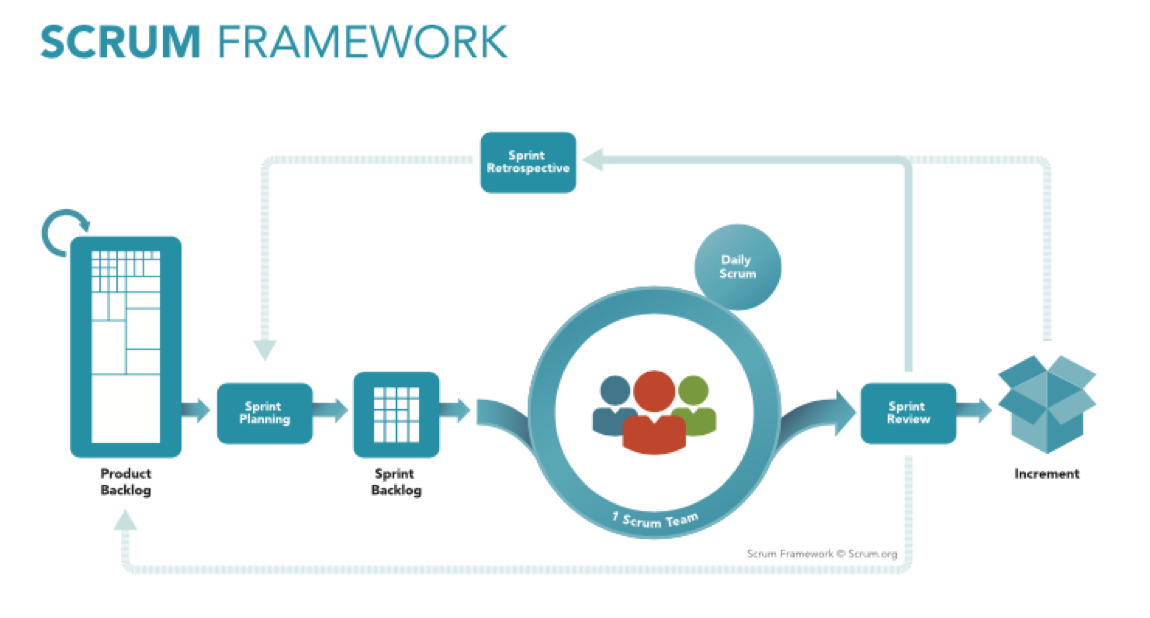
\includegraphics[width=\textwidth,keepaspectratio]{pictures/ScrumFrameworkTest.png}
    		\end{center}
    		\legend{Fonte: https://www.scrum.org/resources/what-is-scrum}
    	\end{figure}

    \section{Utilitários}
    Aqui apresentaremos algumas ferramentas auxiliares que utilizamos para organizar o andamento do projeto.

        \subsection{GitHub}
            GitHub \cite{github} é um servidor de \textit{git}.

        \subsection{Clubhouse}
            Clubhouse \cite{clubhouse} é uma ferramenta online de gerenciamento de projetos de software, provendo funcionalidades interessantes para criar \textit{tasks}, definir \textit{milestones}, verificar o andamento do projeto com \textit{boards} e alguns gráficos. Também provê integração com o \textit{GitHub}.

            \begin{figure}[htb]
                \caption{Board do Formicarium no Clubhouse}
                \begin{center}
                    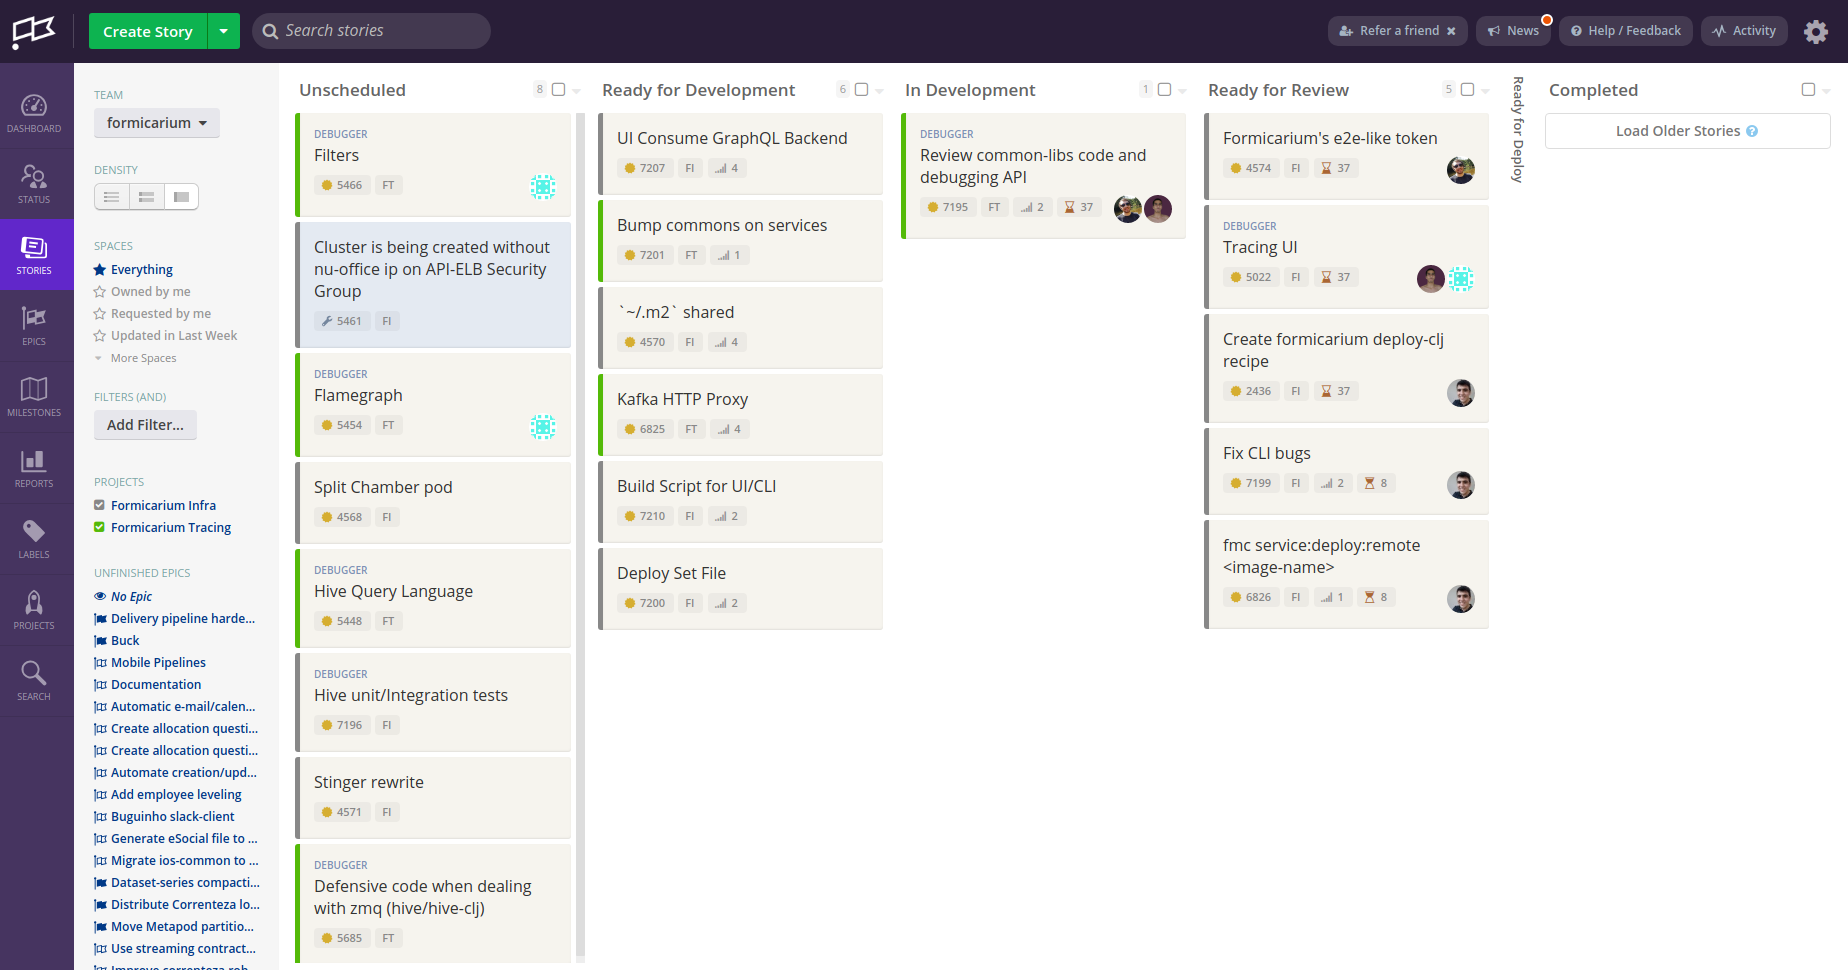
\includegraphics[scale=0.20]{pictures/clubhouse-fmc.png}
                \end{center}
                \label{fig:clubhouse}
                \legend{Fonte: os autores - 2018-11-10}
            \end{figure}

        \subsection{Slack}
            Slack \cite{slack} \textit{software} para equipes que proporciona mensageria instantânea, canais de conversa, \textit{workspaces} e muitas integrações (por exemplo, utilizamos a do \textit{GitHub} para acompanhar os nossos repositórios).
    